\begin{flushleft}
\doublespacing
\subsection{Sekvensdiagram}
Med fodfæste i analysediagrammerne har vi udarbejdet et sekvensdiagram, der illustrerer de overordnede funktioner, der bliver udført af systemer, når man ruller med en terning, rollDice(se figur 5.1.1). Her kaldes altså på metoden diceRoll hos Dice, hvorefter der bliver returneret terningernes øjne. Herefter kalder Game på getPosition hos Player, der returnerer den nuværende spillers position, hvorefter der udregnes en ny position. Når den nye position er fundet, kalder Game landOnField metoden hos Field, som er en abstrakt klasse - metoden er derfor polymorfisk. I følgende paragraffer beskrives hver polymorfisk case.Efter eksekvering af den landOnField tjekker Game for spillets regler hos Rules. Hvis en spiller har mindre en 0 stående på kontoen returnerer Rules en vinder. Herefter opdateres GUIen, hvor der til sidst skifter til næste spiller.
\addlinespace
For nedarvningen ChanceField (se figur 5.1.2) kalder ChanceField på drawChanceCard og executeChanceCard hos ChanceCard. Her trækkes altså et 'tilfældigt' kort, som eksekverer en handling. For at holde diagrammet simpelt viser vi ikke hvert chancekorts udførelse.
\addlinespace
For nedarvningen CustomField står en Player blot stille og der eksekveres altså ikke metoder (se figur 5.1.3).
\addlinespace
For nedarvningen JailField (se figur 5.1.4) kalder JailField på Player, som sætter Player i fængsel, isInJail = true. Hvis en Player ikke besidder et hasGetOutOfJailCard bliver der altså trukket penge fra Player's konto.
\addlinespace
For nedarvningen PropertyField (se figur 5.1.5) kaldes der på Account, setBalance, hvis feltet ikke allerede er købt - her købes feltet så og der trækkes prisen fra kontobalancen, Account. Hvis feltet er købt skal der betales leje, så der kaldes på setBalance hos Account med parametrene currentPlayer og owner, hvor der hhv. subtraheres og adderes med rent.
\addlinespace
I sidste nedarvning, StartField (se figur 5.1.6), kaldes på metoden addBalance hos Account, som tilfører currentPlayer 2 point til kontoen.
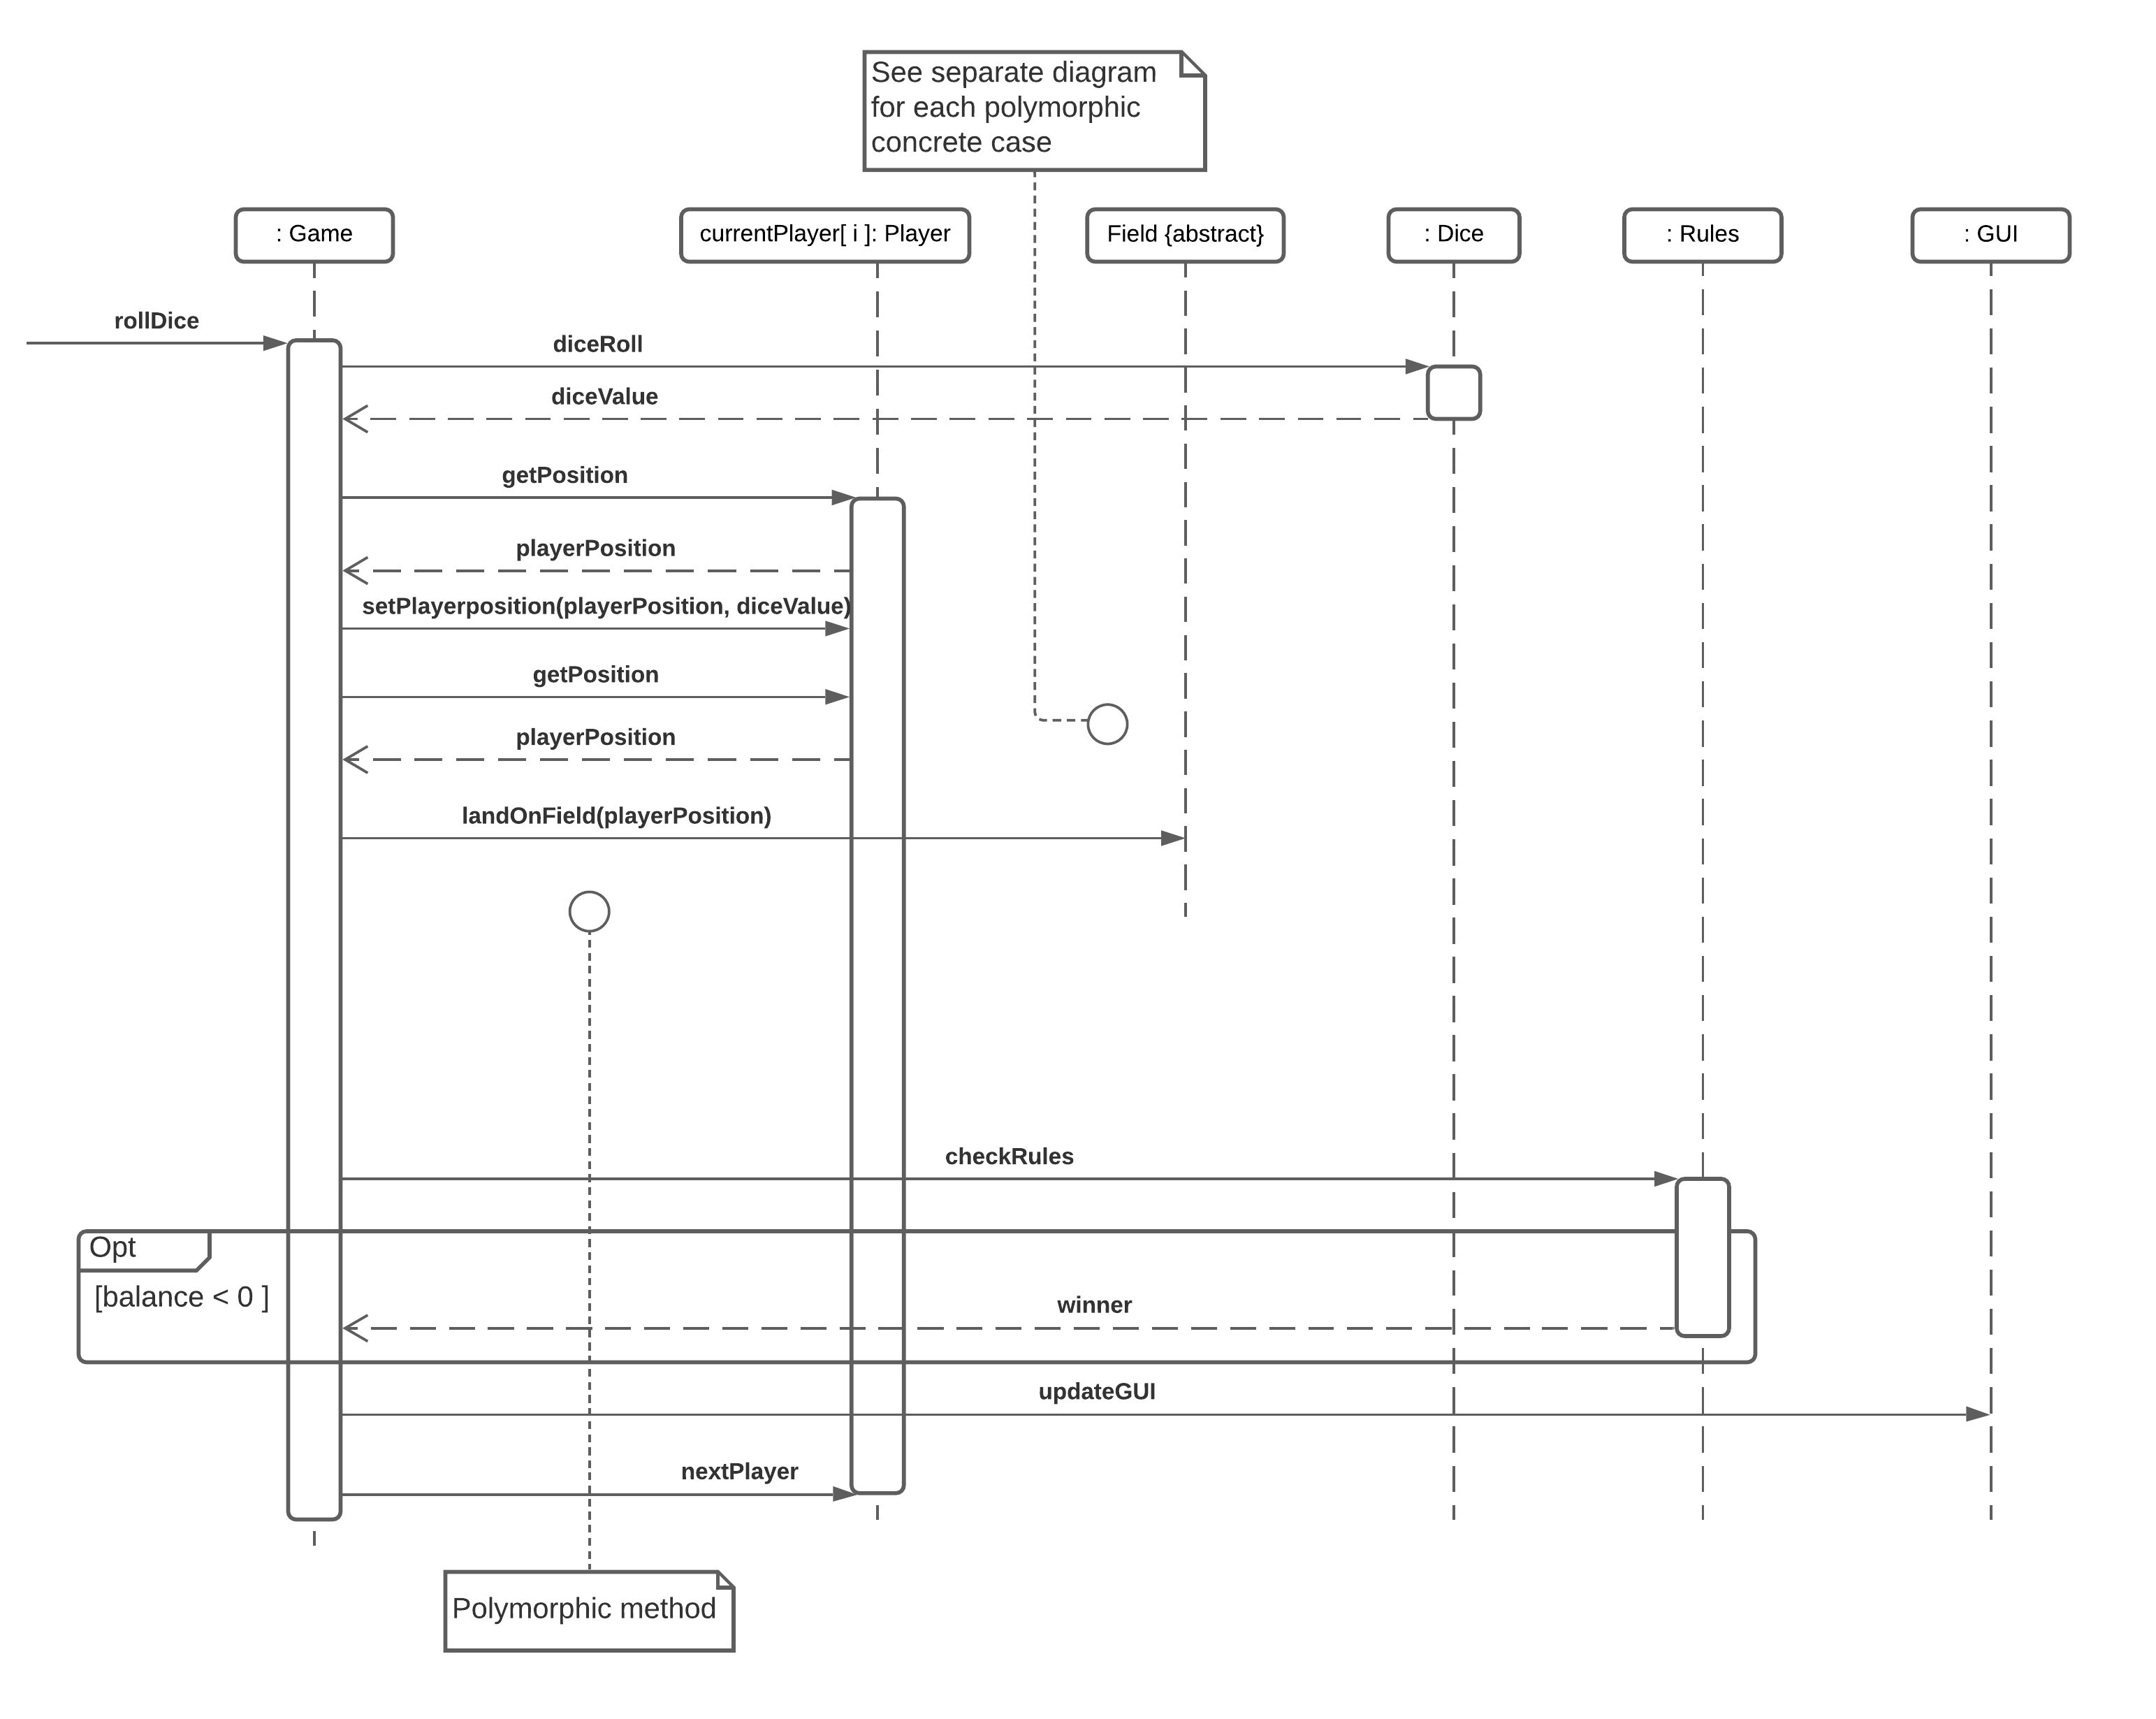
\includegraphics[width=1\textwidth]{Report/figures/Sekvensdiagram1.png}~\\[0cm]
Figur 5.1.1. Sekvensdiagram over rollDice som use-case.

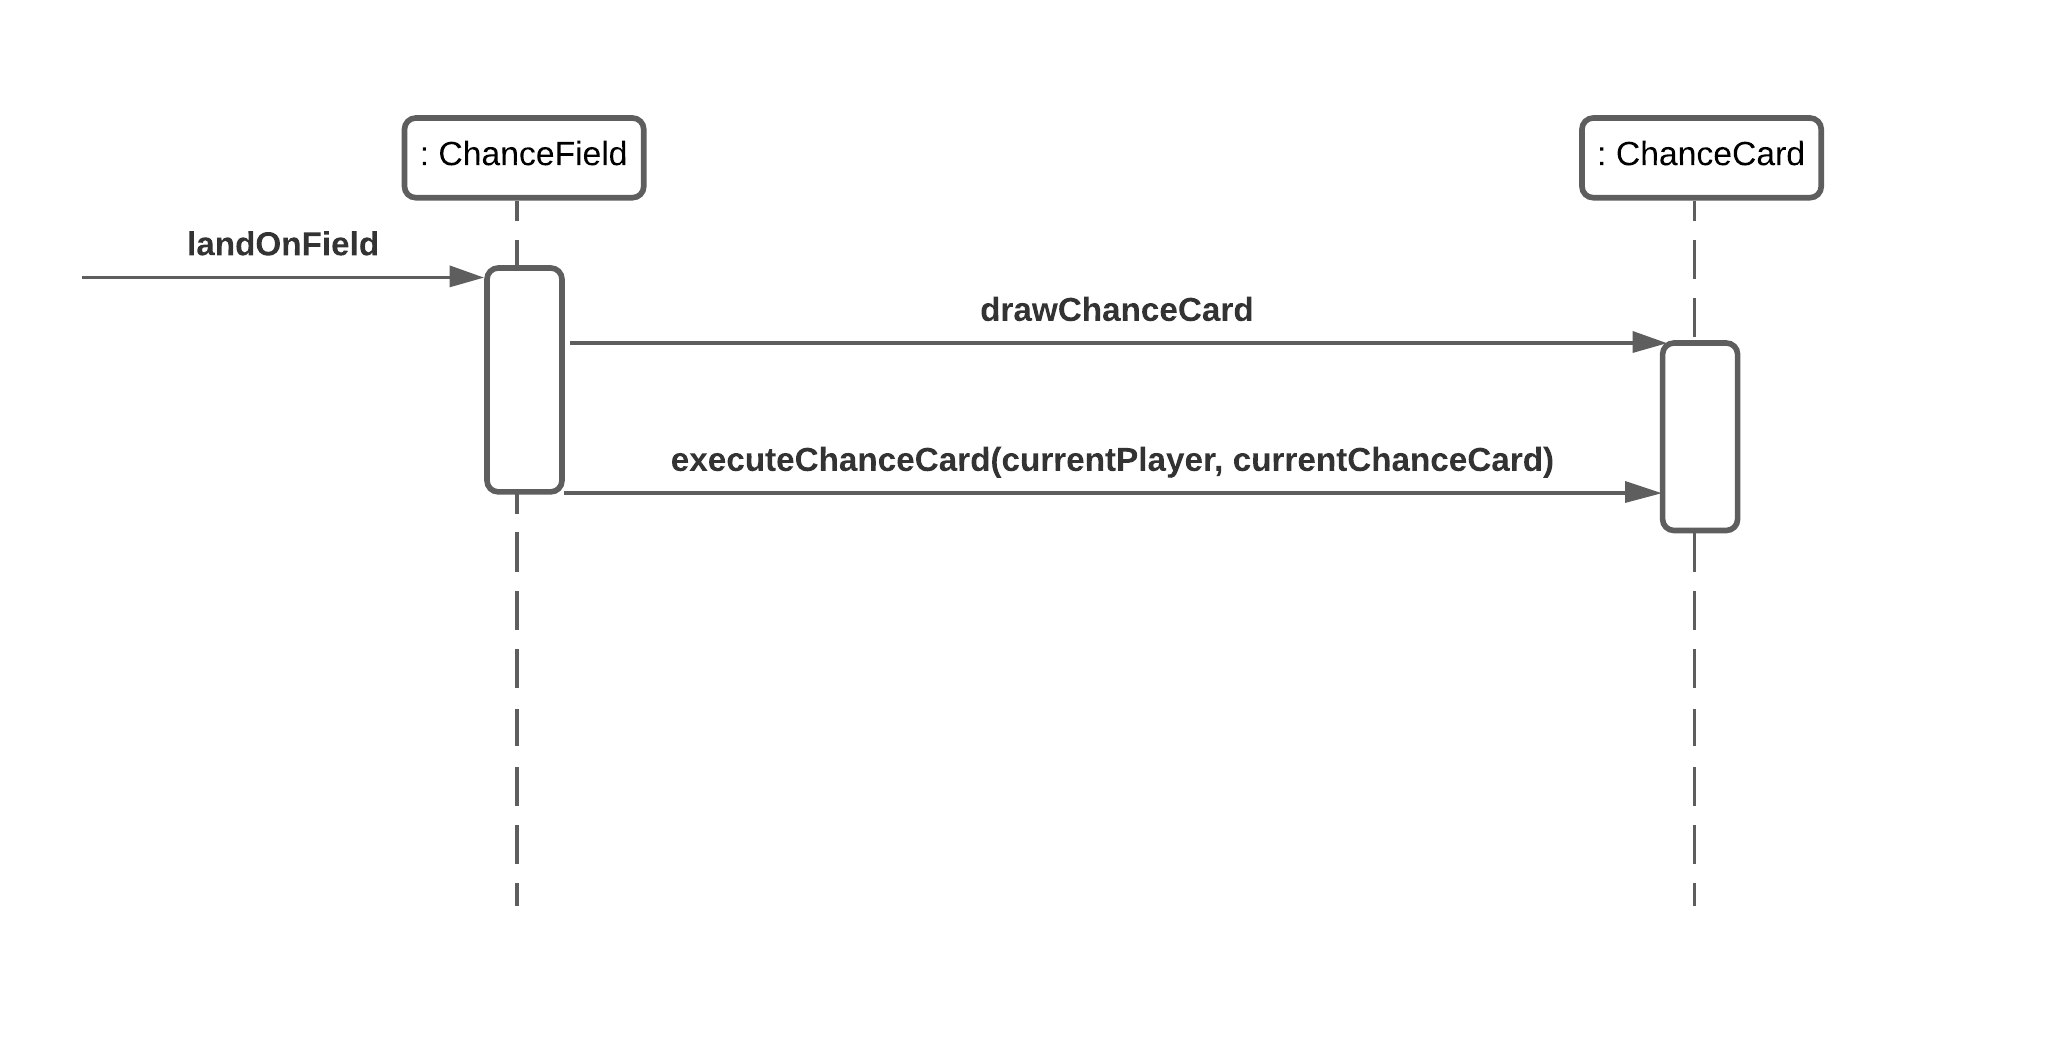
\includegraphics[width=0.9\textwidth]{Report/figures/Sekvensdiagram_ChanceField.png}~\\[0cm]
Figur 5.1.2. Sekvensdiagram over polymorphism af metoden landOnField for ChanceField.


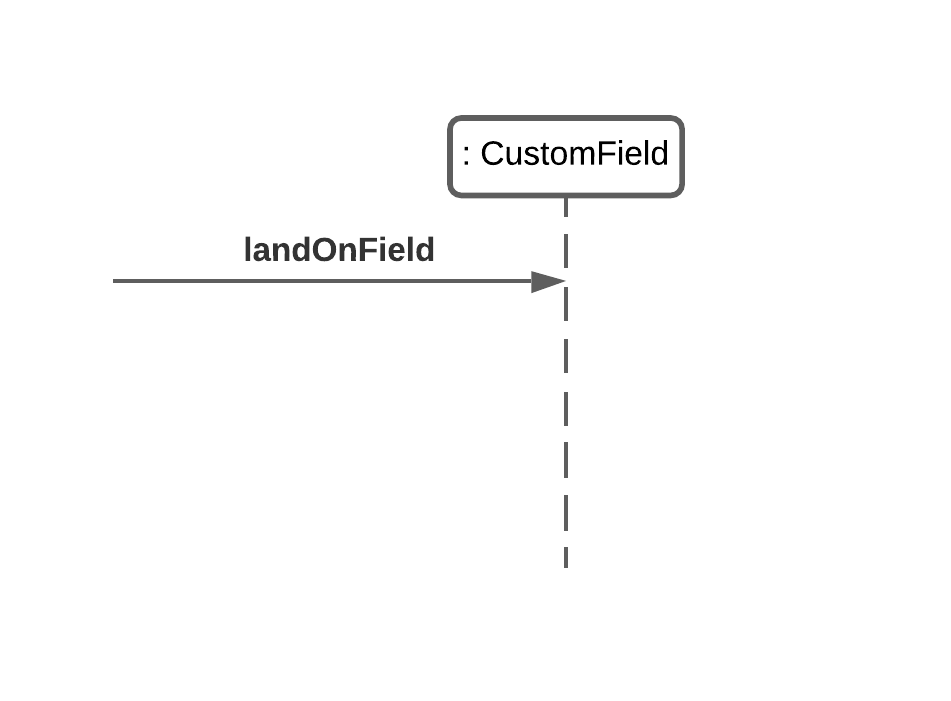
\includegraphics[width=0.9\textwidth]{Report/figures/Sekvensdiagram_CustomField.png}~\\[0cm]
Figur 5.1.3. Sekvensdiagram over polymorphism af metoden landOnField for CustomField.


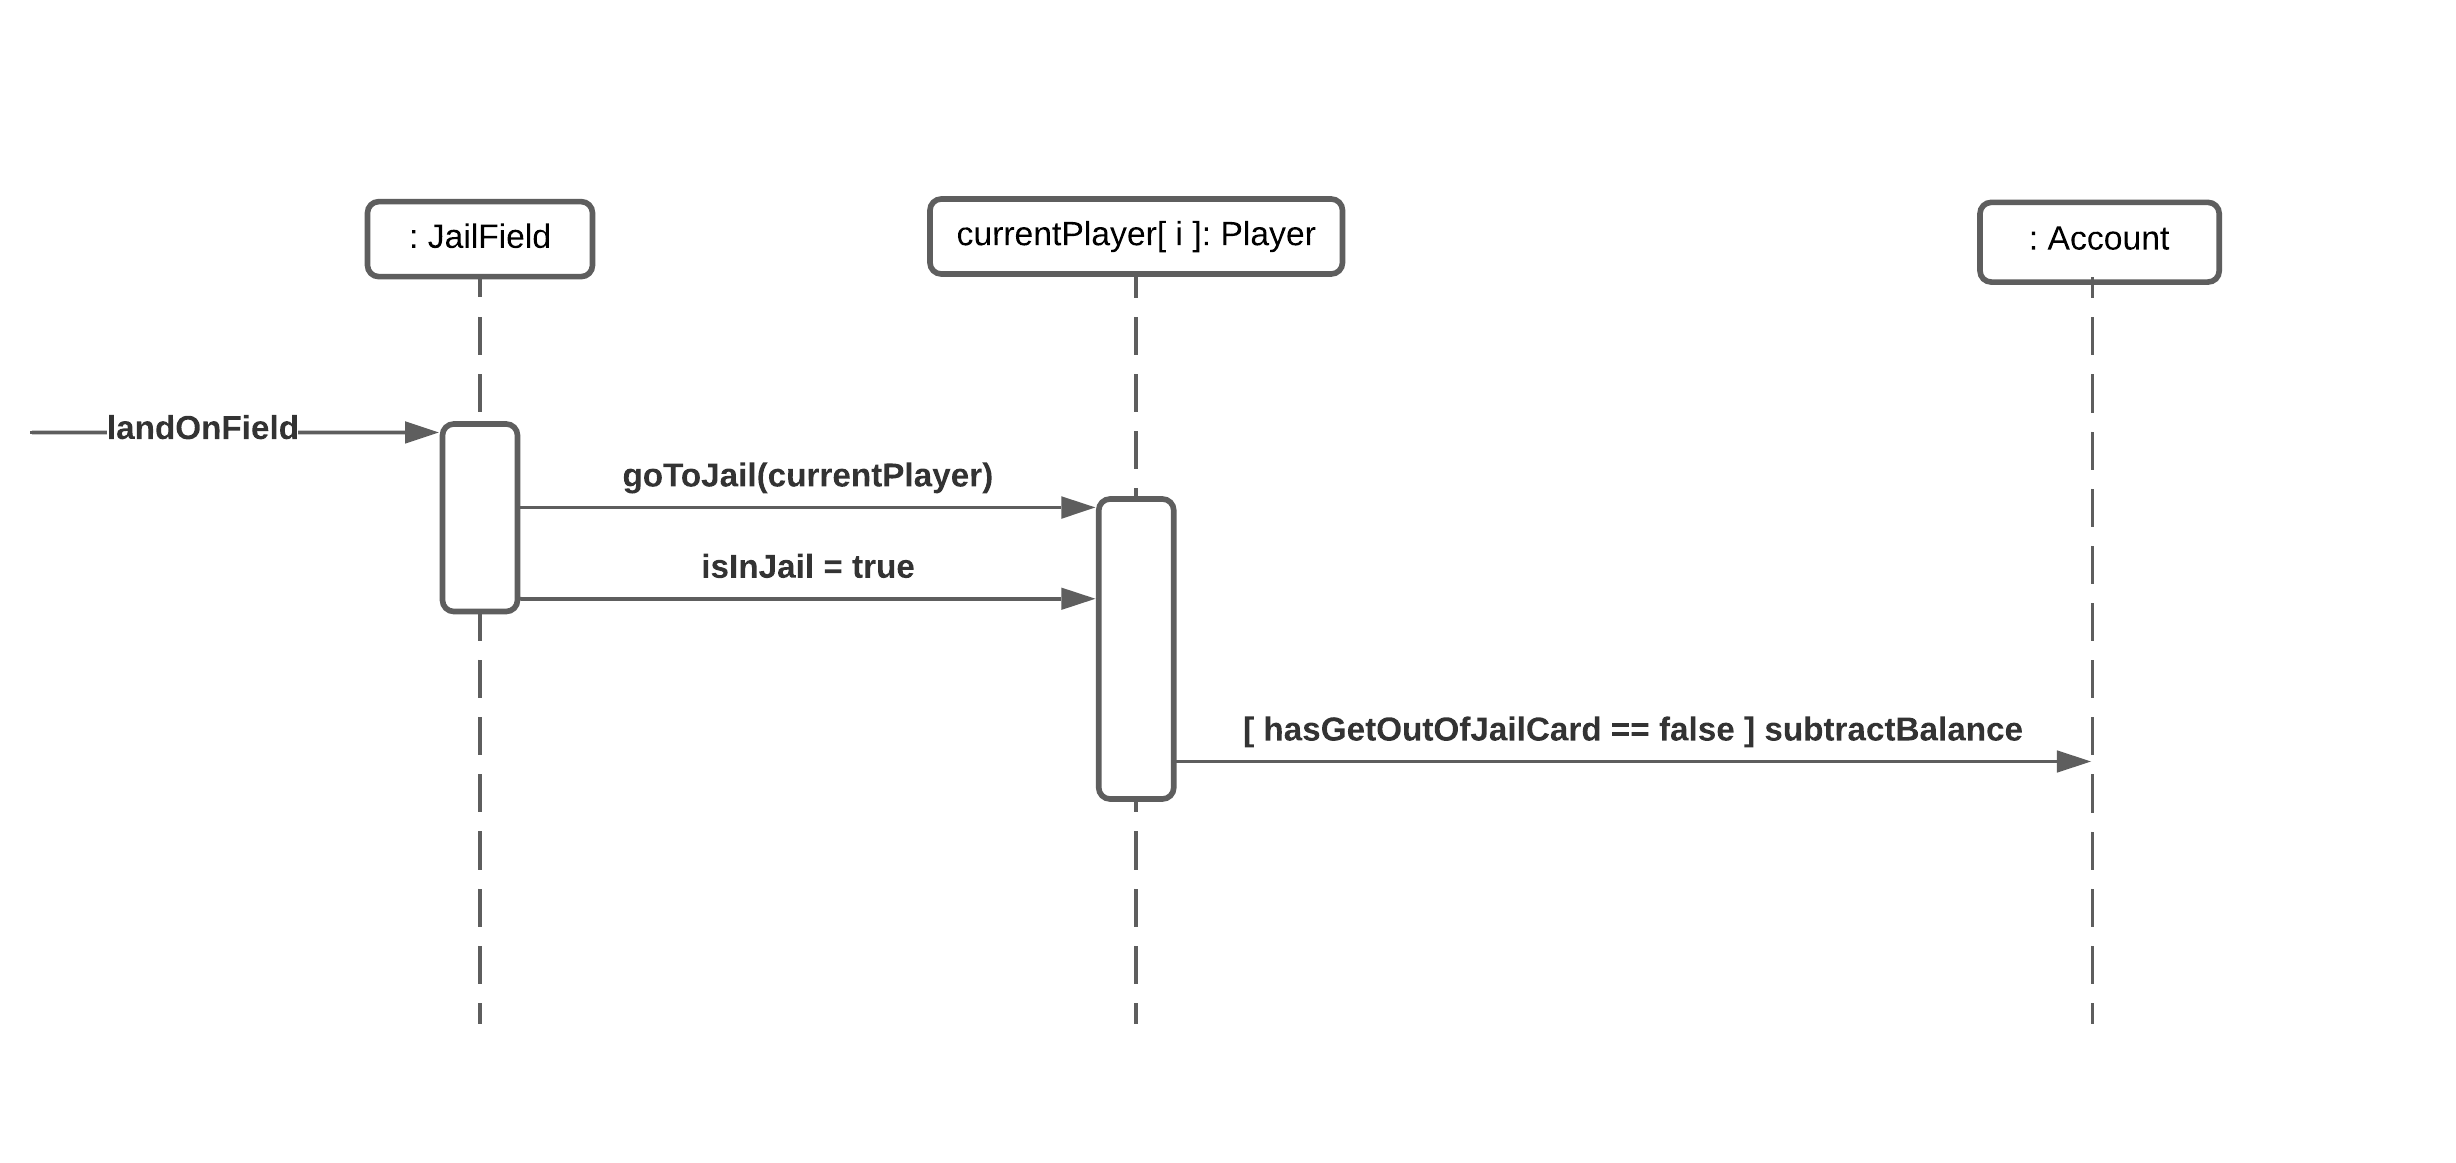
\includegraphics[width=0.9\textwidth]{Report/figures/Sekvensdiagram_JailField.png}~\\[0cm]
Figur 5.1.4. Sekvensdiagram over polymorphism af metoden landOnField for JailField.


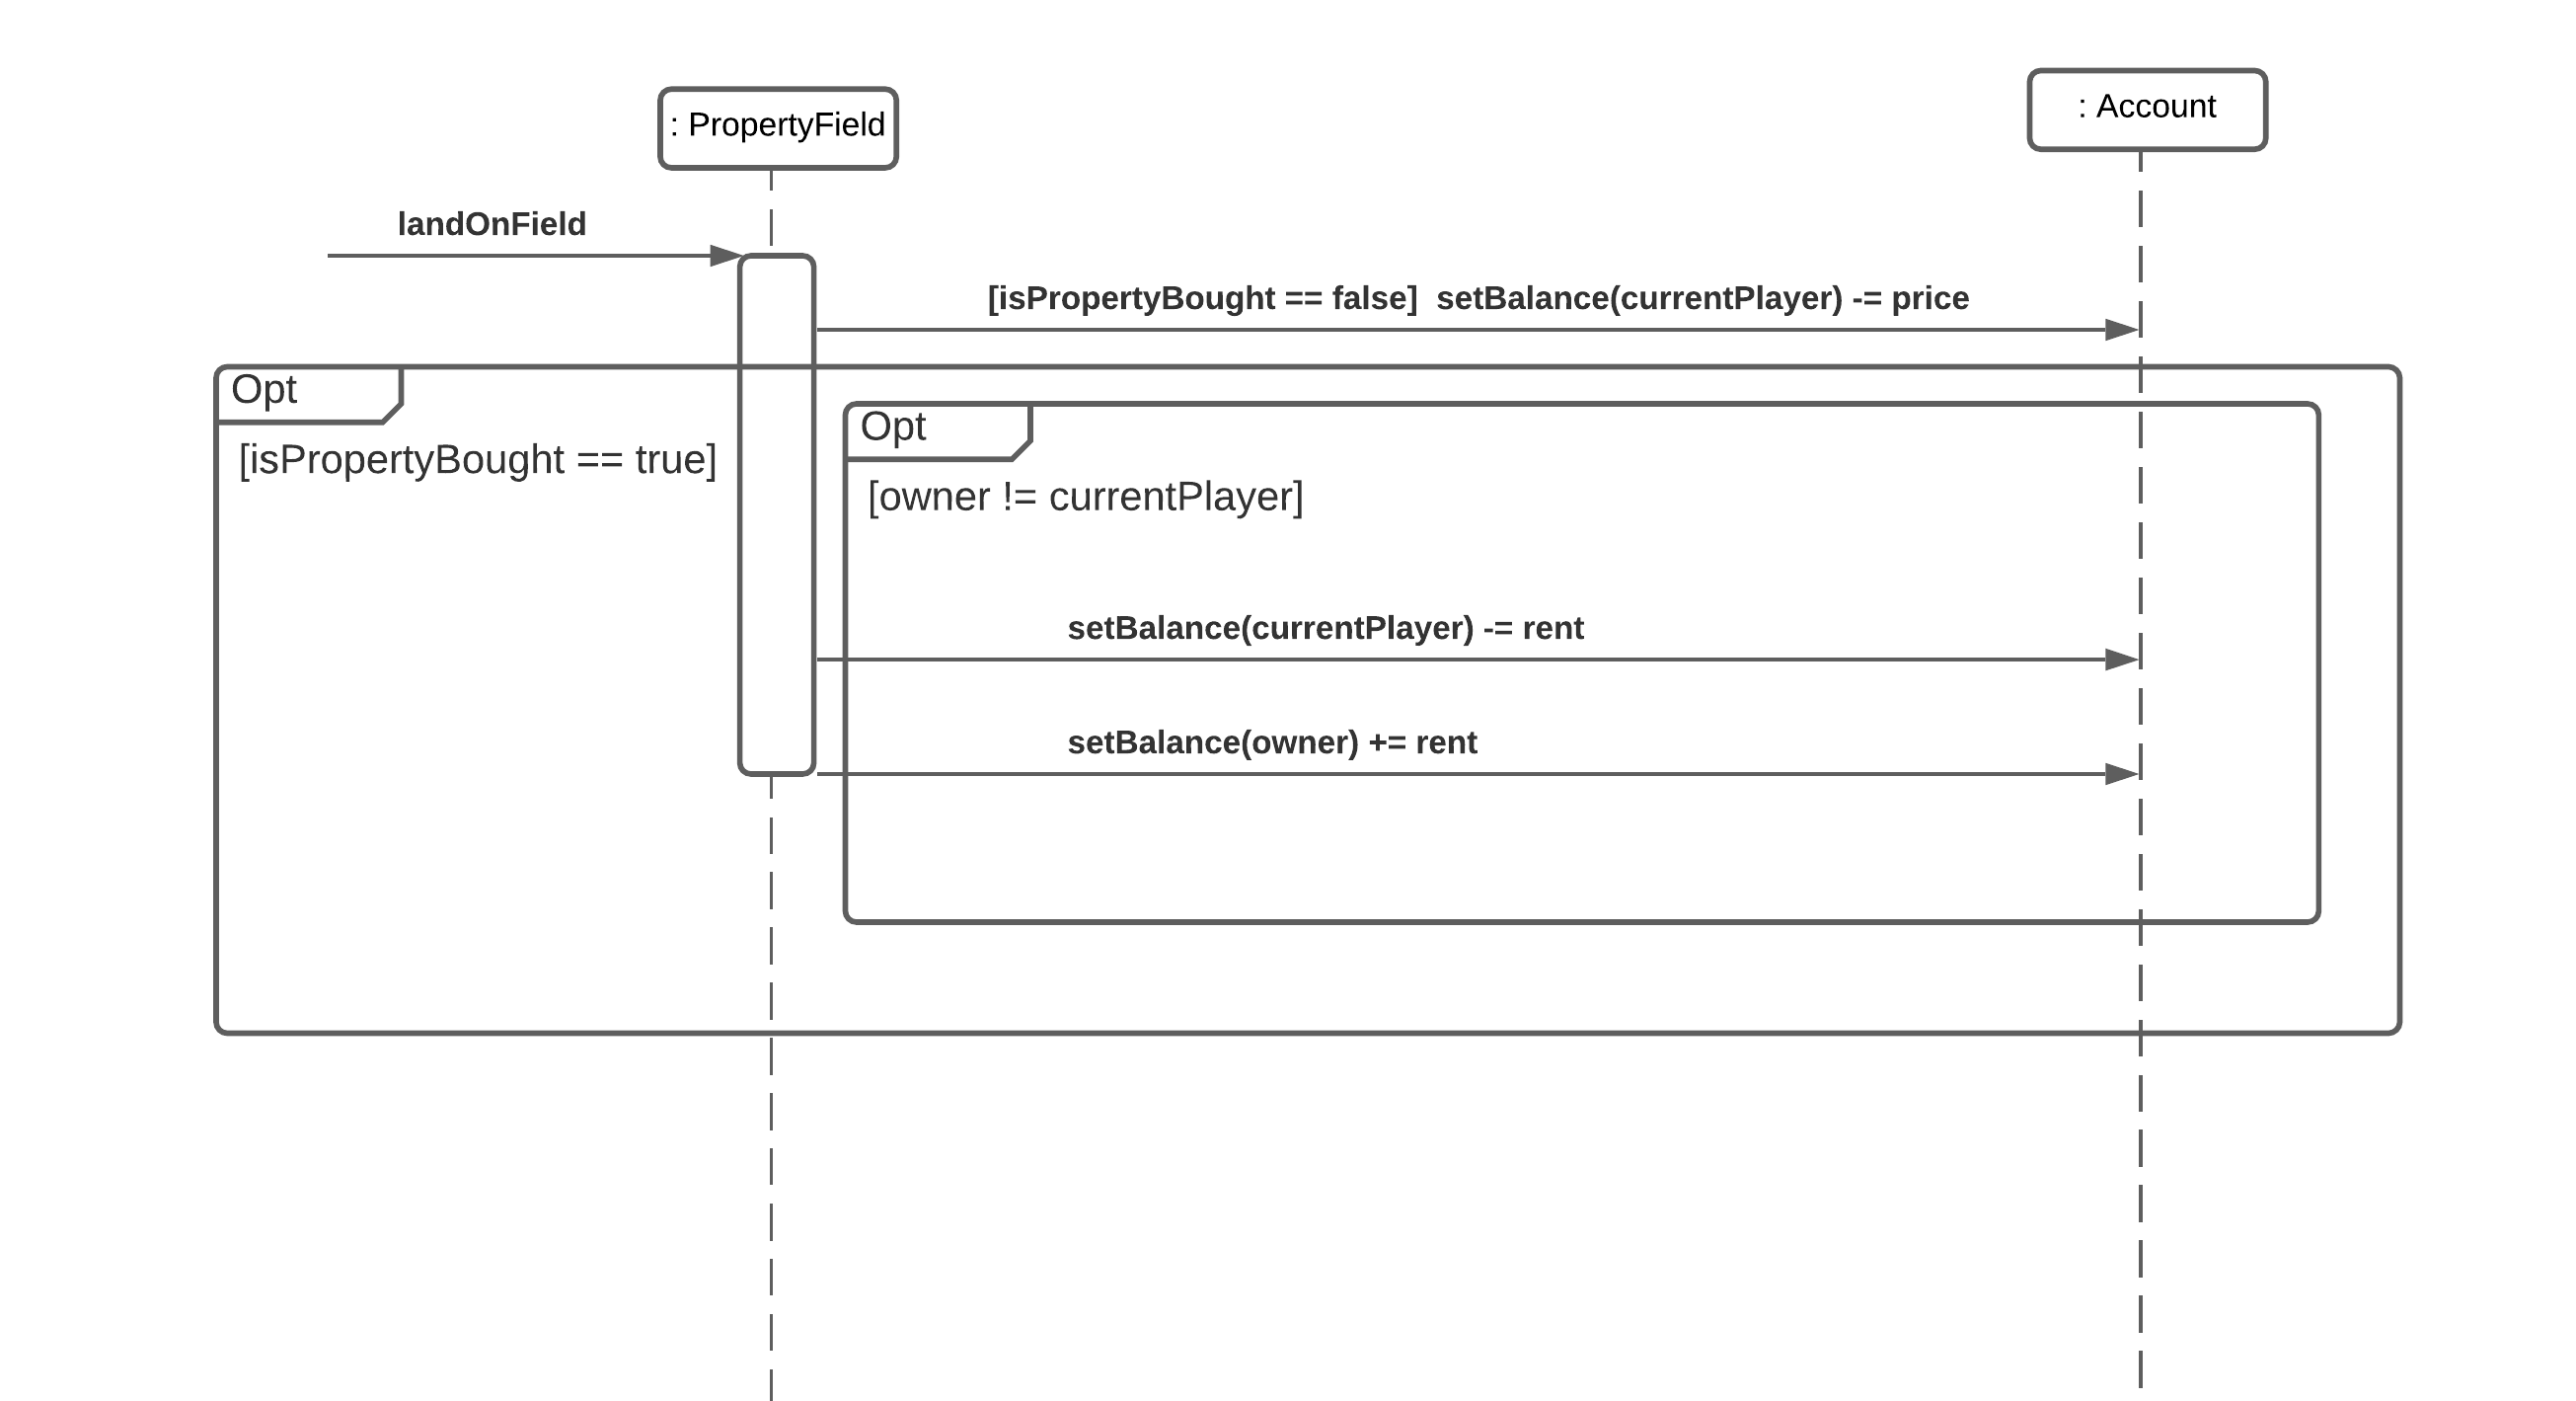
\includegraphics[width=0.9\textwidth]{Report/figures/Sekvensdiagram_PropertyField.png}~\\[0cm]
Figur 5.1.5. Sekvensdiagram over polymorphism af metoden landOnField for PropertyField.


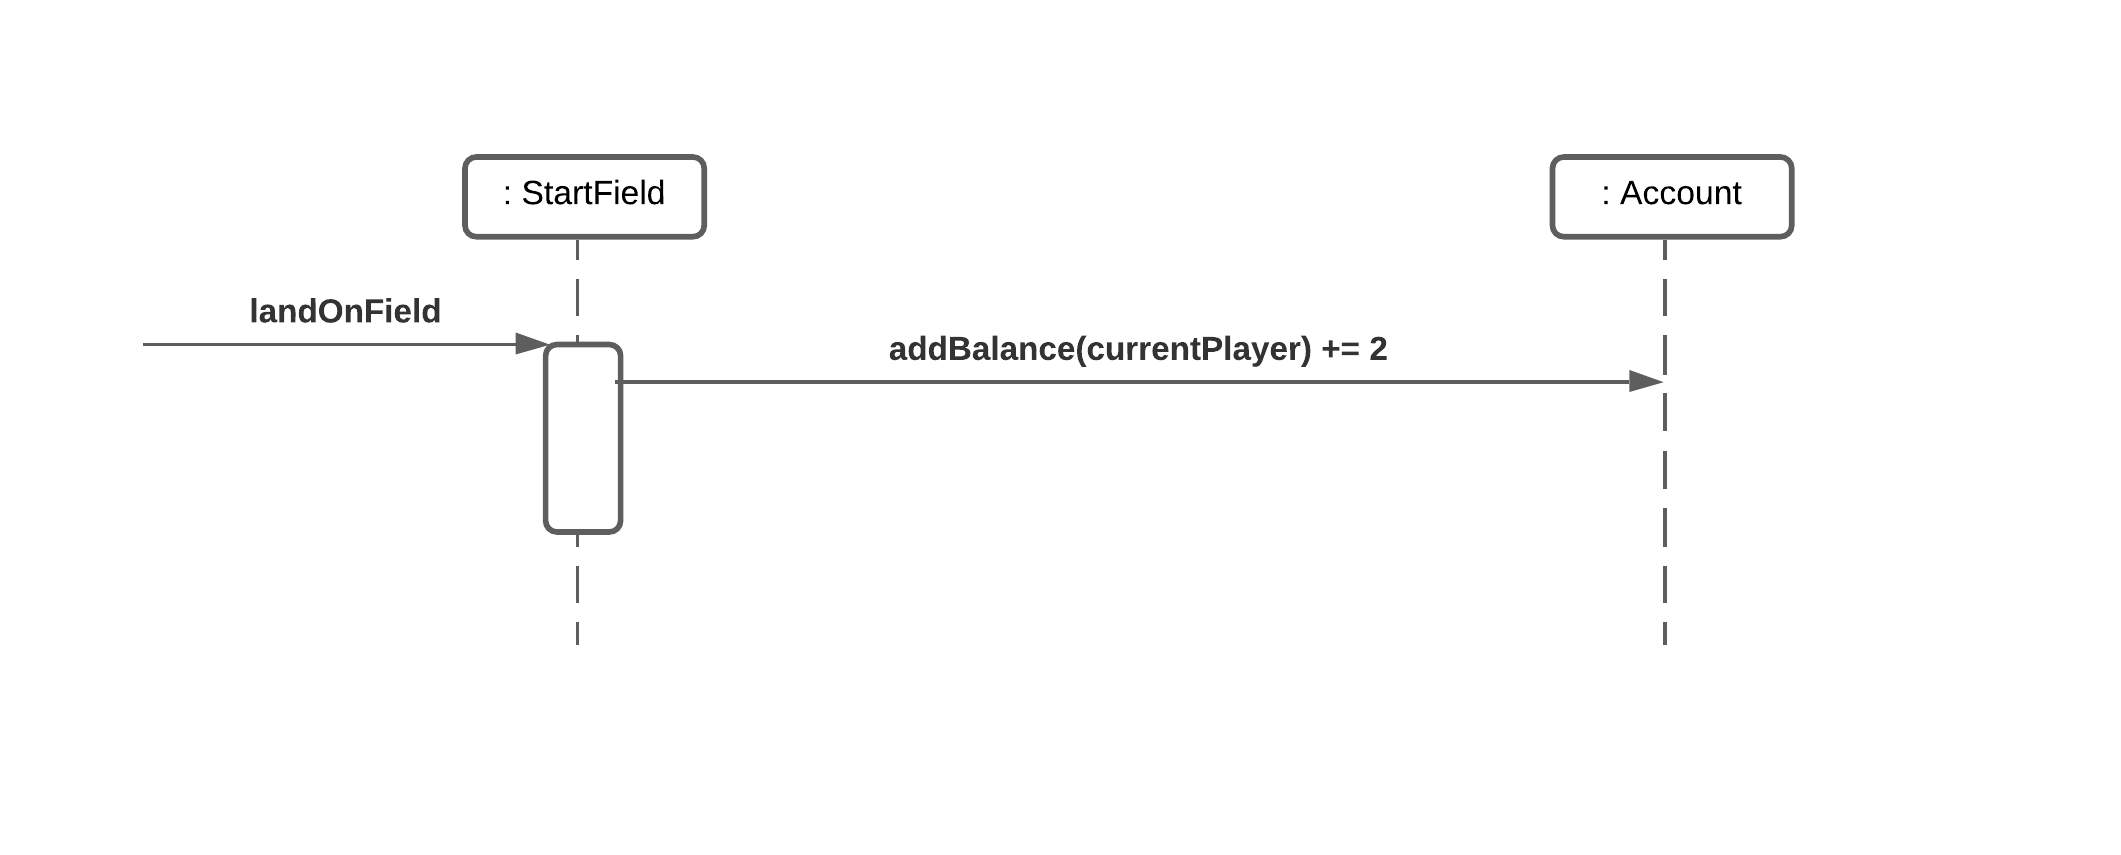
\includegraphics[width=0.9\textwidth]{Report/figures/Sekvensdiagram_StartField.png}~\\[0cm]
Figur 5.1.6. StartField over polymorphism af metoden landOnField for ChanceField.
\subsection{Designmønster GRASP}
I dette afsnit beskriver vi kort, hvordan vores design har overholdt GRASP principper. Her refereres der til designklassediagrammet (se figur 5.2.1) uden at danne en fyldestgørende beskrivelse af dette diagram. For en fyldestgørende beskrivelse, se afsnit 5.3.
\subsection{Designklassediagram}
\begin{center}
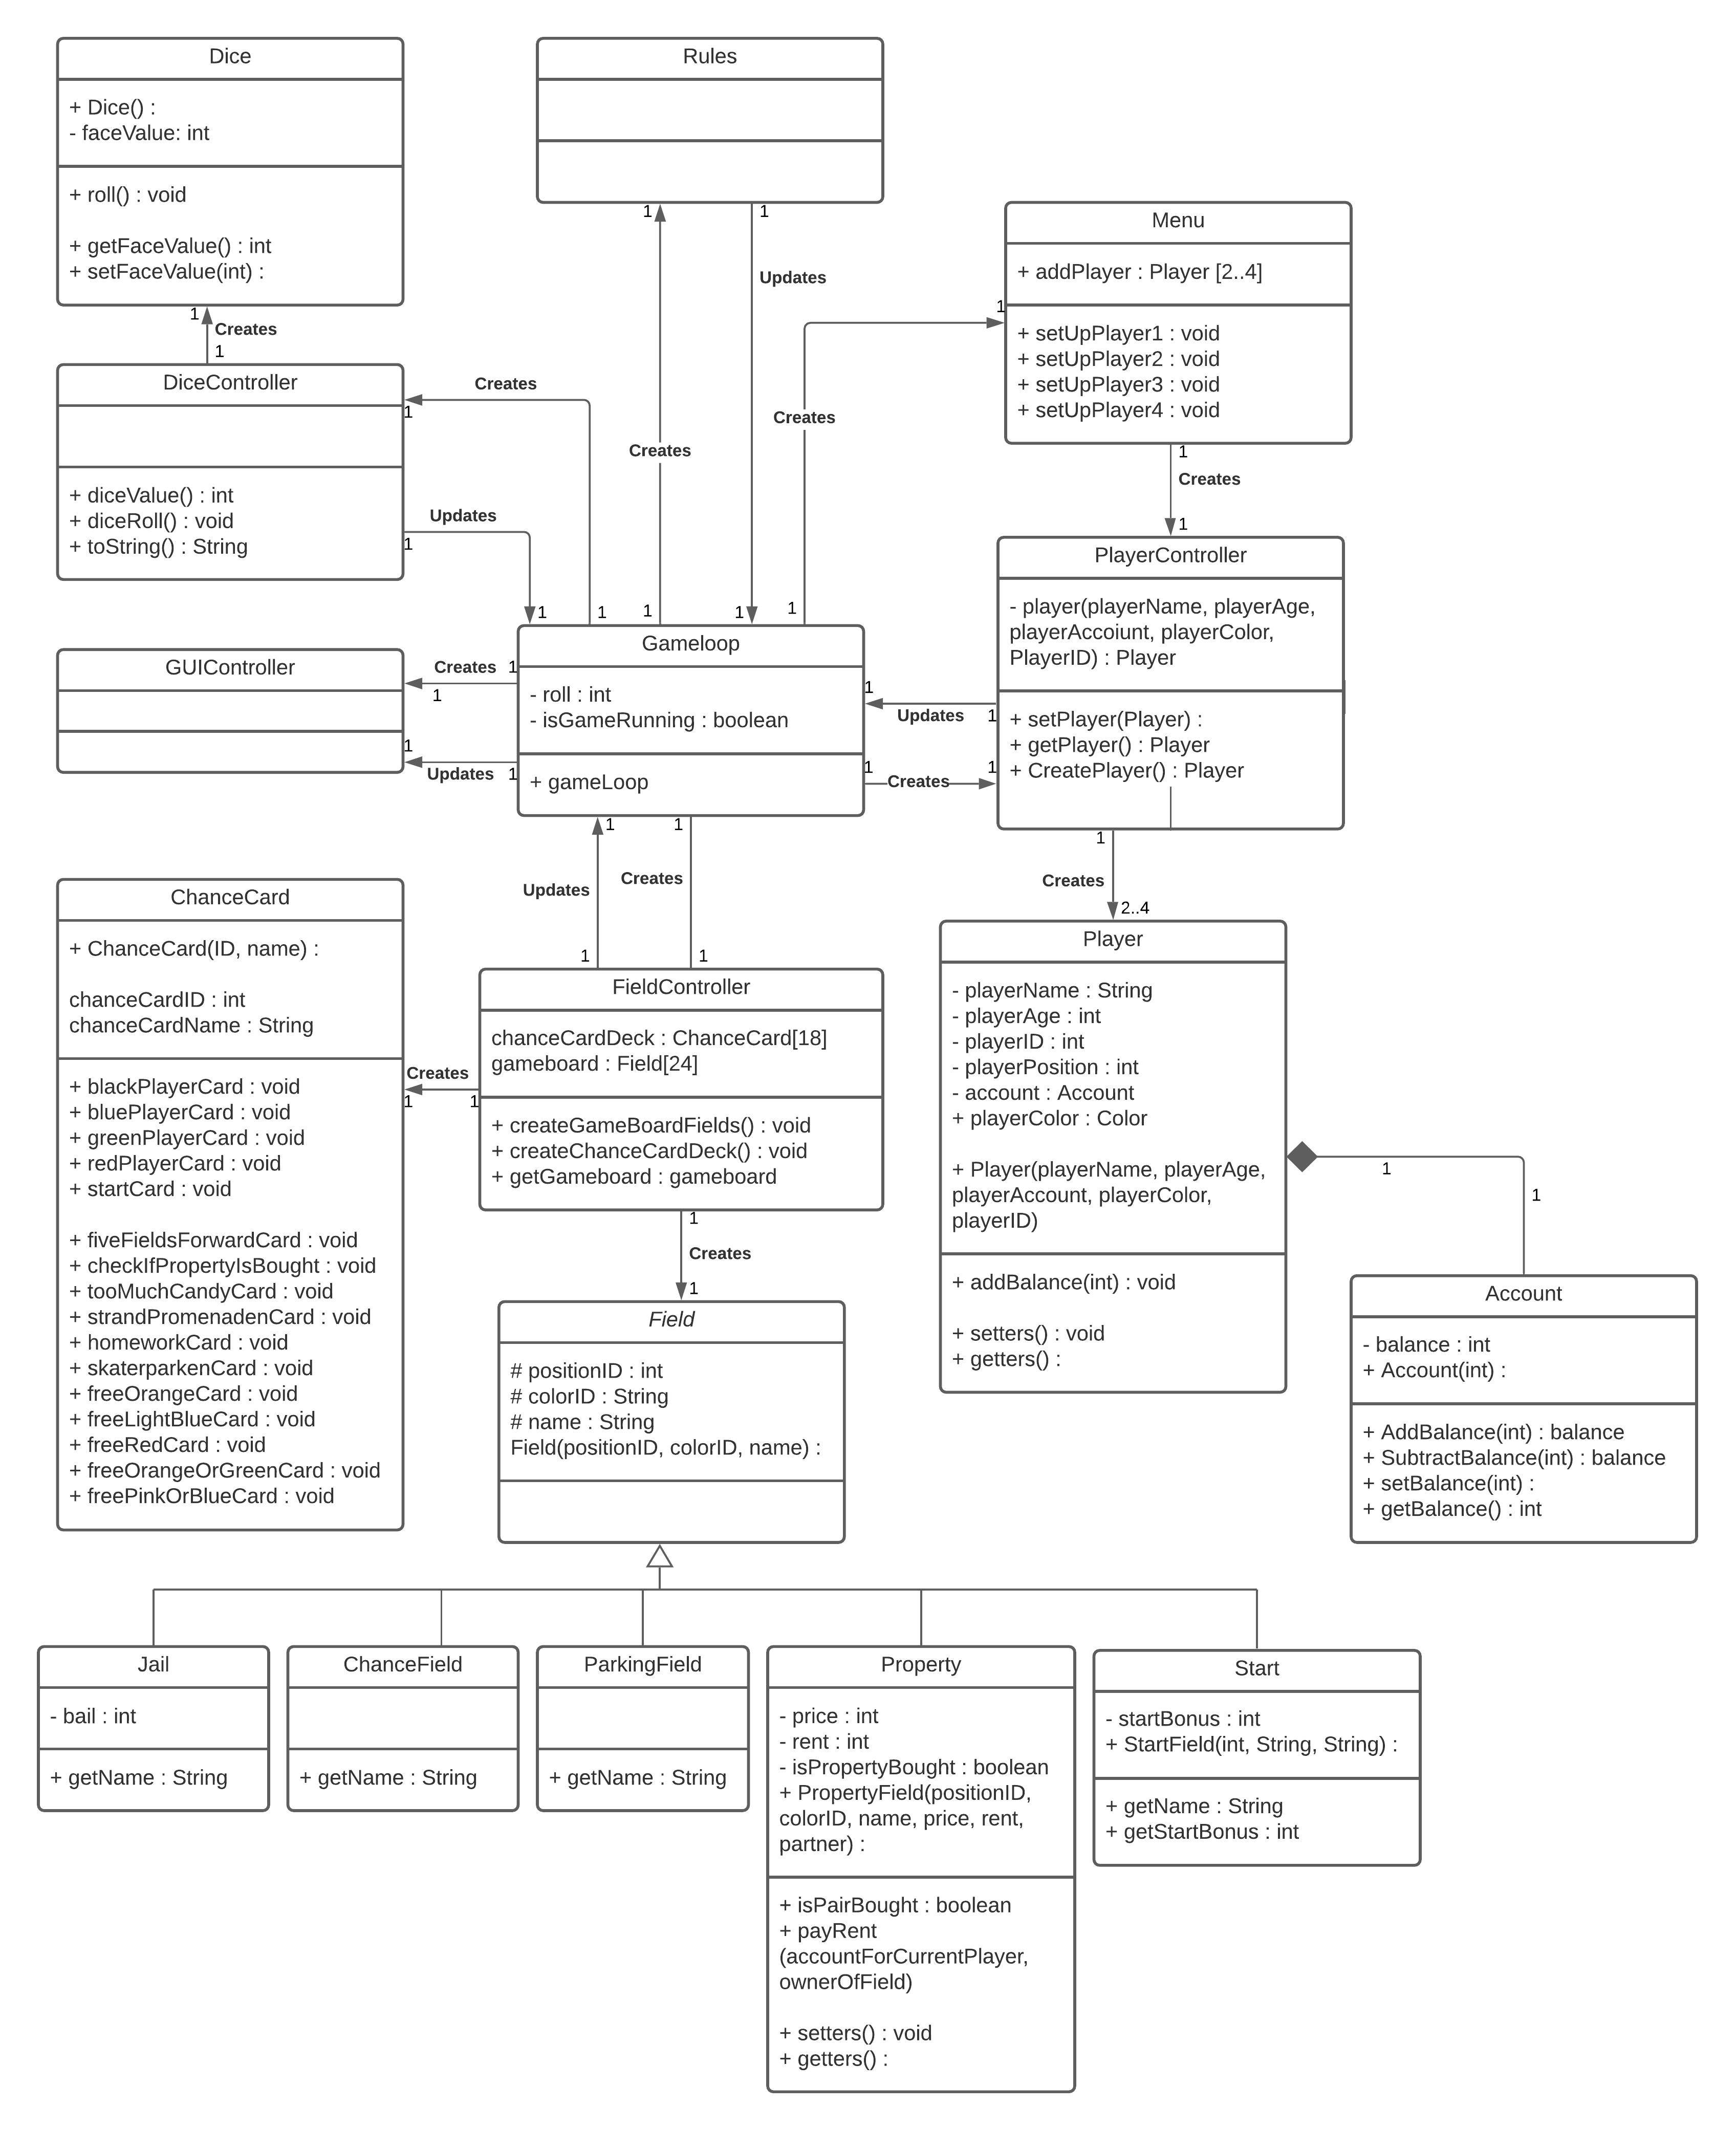
\includegraphics[width=1\textwidth]{Report/figures/Class Diagram.png}~\\[0cm]
\end{center}
Figur 5.2.1. Designklassediagram over Monopoly Junior spillet.
\end{flushleft}